%-----------------------------------------------
% Dateiname: TYPO3CMS.tex
% Autor    : Stefano Kowalke <blueduck@gmx.net>
% Lizenz   : BSD
%-----------------------------------------------
\section{TYPO3 CMS}
\label{sec:typo3cms}
\subsection{Geschichte}
\label{subsec:historyTypo3}
TYPO3 CMS ist ein \gls{wcms} und wurde von dem dänischen Programmierer Kaspar Skårhøj im Jahr 1997 zunächst für seine Kunden entwickelt - im Jahr 2000 von ihm unter der \gls{gpl2} veröffentlicht. Dadurch fand es weltweit Beachtung und erreichte eine breite Öffentlichkeit. Laut der Website T3Census\footnote{\url{http://t3census.info/}} gab es am 7. April 2014 208561 Installationen von TYPO3 CMS.
\\
\\
\begin{figure}[h!]
	\startchronology[startyear=1995, stopyear=2015]
	\chronoevent{1997}{Beginn der Entwicklung}
	\chronoevent[markdepth=45pt]{2001}{Version 3.0}
	\chronoevent{2006}{Versoin 4.0}
	\chronoevent[markdepth=25pt]{2011}{Versoin 4.5 LTS}
	\chronoevent[markdepth=55pt]{2014}{Version 6.2 LTS}
	\stopchronology
	\caption{Zeitachse der TYPO3 CMS Entwicklung}
\end{figure}

Im Jahr 2012 entschied sich das Projekt zu einer Änderung in der Namesgebung:
\begin{itemize}
	\item aus TYPO3 v4\footnote{Damit ist das von Skårhøj entwickelte \gls{cms} gemeint, welches den 4.x Zweig des Projekts darstellt.} wurde TYPO3 CMS
	\item aus FLOW3 wurde TYPO3 Flow
	\item und aus TYPO3 5.0 / TYPO3 Phoenix wurde TYPO3 Neos
\end{itemize}

Diese Änderung wurde notwendig, da schon länger abzusehen war, dass TYPO3 Phoenix nicht den Nachfolger von TYPO3 v4 darstellt. Somit war die Entwicklung von TYPO3 v4 in dem Versionszweig 4.x gefangen und es konnten keine neuen Features eingebaut oder veraltete Funktionen entfernt werden. Durch dieses neue Schema bekommt der Name "TYPO3" die Bedeutung einer Dachmarke zuteil, während "TYPO3 CMS", "TYPO3 Flow" und "TYPO3 Neos" Produkte innerhalb der TYPO3 Familie darstellen. Im weiteren Verlauf dieser Arbeit werden ausschließlich die neuen Namen verwendet.

Heute kümmert sich ein Team um die Entwicklung von TYPO3 CMS und eines um TYPO3 Flow und TYPO3 Neos. Dahinter steht keine Firma, wie es bei anderen Open Source Projekten wie Drupal (Acquia) oder Wordpress (Automattic) vorzufinden ist, sondern die \gls{t3assoc}. Die \gls{t3assoc} ist ein gemeinnütziger Verein und wurde 2004 von Kaspar Skårhøj und anderen Entwicklern gegründet um als Anlaufstelle für Spenden zu dienen, die die langfristige Entwicklung von TYPO3 sicherstellen sollen. Die Spenden werden in Form von Mitgliedsbeiträgen erhoben.\footnote{\url{http://association.typo3.org/}}

\subsection{Definition}
TYPO3 CMS ist ein klassisches \gls{cms}, welches auf die Erstellung, die Bearbeitung und das Publizieren von Inhalten im Intra- oder Internet spezialisiert ist und es somit per Definition zu einem \gls{wcms} macht.

Daneben findet man auch die Bezeichnung \gls{ecms}\footnote{\url{http://www.typo3.org}}, was als Hinweis auf den Einsatz des Systems für mittel- bis große Webprojekte dient.

\subsection{Architektur und Aufbau von TYPO3 CMS}
\label{subsec:architectureTypo3}
Im folgenden werden die grundlegenden Konzepte von TYPO3 CMS vorgestellt. Dort wo es für das weitere Verständnis notwendig ist, wird tiefer in das Thema eingestiegen. Ansonsten werden die Konzepte lediglich angerissen um einen generellen Überblick zu erhalten.

\subsubsection{Webstack als Basis}

TYPO3 CMS wurde in \gls{php} - basierend auf dem Konzept der Objektorientierung - geschrieben und ist damit auf jeder Plattform lauffähig, die über einem \gls{php} Interpreter verfügt. Die Version 6.2 von TYPO3 CMS benötigt mindestens \gls{php} 5.3.7.

\gls{php} bildet zusammen mit einem Apache Webserver und einer MySQL Datenbank den sogenannten Webstack, der abhängig von dem eingesetzten Betriebssystem MAMP (OSX / {\bfseries M}ac), LAMP ({\bfseries L}inux) oder WAMP ({\bfseries W}indows) heißt.

In der Standardeinstellung kommt MySQL als Datenbank zum Einsatz - durch die Systemextension\footnote{Eine kurze Einführung in die verschiedenen Arten von Extension findet sich im Kapitel \ref{subsubsec:sysext}} \textit{DBAL} können jedoch auch Datenbanken anderer Hersteller angesprochen werden. Eine genaue Analyse dieser Extension erfolgt im Kapitel~\ref{extDBAL}[Kapitel zur Analyse von ext:DBAL einfügen].

\subsubsection{Ansichtssache}
Aus Anwendersicht teilt sich TYPO3 CMS in zwei Bereiche:

\begin{itemize}
	\item das Backend\\
		stellt die Administrationsoberfläche dar. Hier erstellen und verändern Redaktuere die Inhalte; während Administratoren das System von hier aus konfigurieren
	\item das Frontend\\
		stellt die Website dar, die ein Besucher zu Gesicht bekommt.
\end{itemize}
(vgl. \cite[S. 5]{book:dulepovTypo32008})

\subsubsection{Der Systemkern und die \gls{api}s}
\label{basics:typo3:subsubsec:coreAndApi}
TYPO3 CMS besteht aus einem Systemkern, der lediglich grundlegende Funktionen zur Datenbank-, Datei- und Benutzerverwaltung zu Verfügung stellt. Dieser Kern ist nicht monolithisch aufgebaut, sondern besteht aus Systemextensions. (vgl. \cite[S. 32]{book:laborenzTypo32006})

\begin{figure}[H]
	\centering
	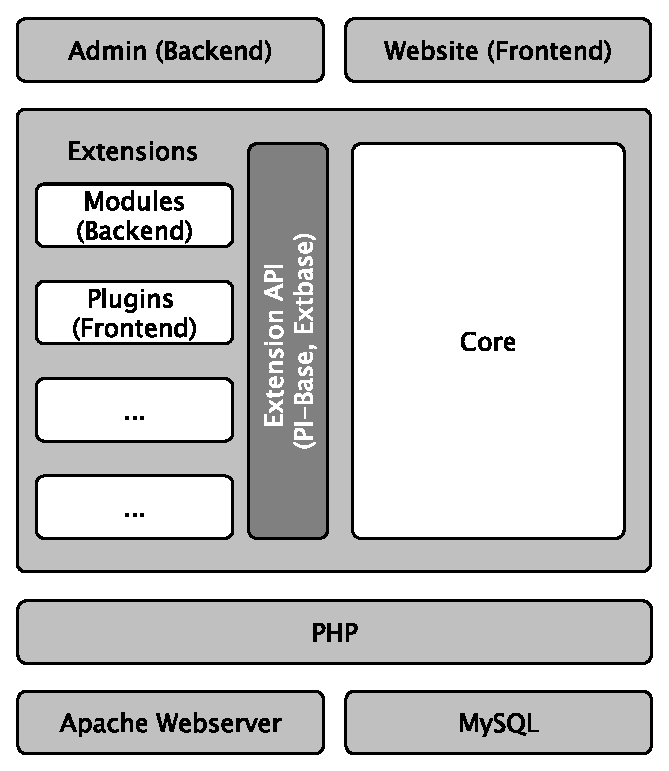
\includegraphics[scale=0.77]{diagrams/TYPO3Architecture.eps}
	\caption{Schematischer Aufbau von TYPO3}
	\label{fig:typo3Architecture}
\end{figure}

Die Gesamtheit aller von TYPO3 CMS zur Verfügung gestellten \gls{api}s, wird als die \mbox{\textit{TYPO3 API}} bezeichnet. Diese kann - analog zum Konzept von Backend und Frontend - in eine \mbox{\textit{Backend \gls{api}}} und eine \mbox{\textit{Frontend \gls{api}}} unterteilt werden kann. Die Aufgabe der Frontend \gls{api} ist die Zusammenführung der getrennt vorliegenden Bestandteile (Inhalt, Struktur und Layout) aus der Datenbank oder dem Cache zu einer HTML-Seite. Die Backend \gls{api} stellt Funktionen zur Erstellung und Bearbeitung von Inhalten zur Verfügung. (vgl. \cite[S. 5 ff.]{book:dulepovTypo32008})

Die \gls{api}s, die keiner der beiden Kategorien zugeordnet werden kann, bezeichnet Dulepov \cite[S. 5 ff.]{book:dulepovTypo32008} als \mbox{\textit{Common-\gls{api}}}. Die Funktionen der Common-\gls{api} werden von allen anderen \gls{api}s genutzt. Ein Beispiel dafür stellt die Datenbank \gls{api} dar, welche in der Regel nur einfache Funktionen wie das Erstellen, Einfügen, Aktualisieren, Löschen und Leeren\footnote{CRUD - {\bfseries C}reate, {\bfseries R}etrieve, {\bfseries U}pdate und {\bfseries D}elete} von Datensätzen bereitzustellen hat. Würde man je eine Datenbank \gls{api} für das Frontend und das Backend zur Verfügung stellen, bricht man eine wichtige Regel der Objekt-orientierten Programmierung - Don't repeat yourself. Dieser - mit hoher Wahrscheinlichkeit - redundante Code würde die Wartbarkeit des Programms verschlechtern und die Fehleranfälligkeit erhöhen.

Auf die aktuelle Datenbank-\gls{api} wird in Kapitel \ref{currentSituation}[KAPITEL zur Analyse der aktuellen Situation einfügen] näher eingegangen.

\subsubsection{Verzeichnisstruktur}

Im Gegensatz zu früheren TYPO3 CMS Versionen gibt es kein \mbox{\textit{Dummy-Package}}\footnote{Damit ist ein weitgehend leeres Paket gemeint, dass alle Dateien enthält die im Web\-root des Servers laufen sollen. Es stellt einen Container für die spätere Website dar.} mehr. Ab Version 6.2 enthält der Download lediglich den TYPO3 CMS Kern in Form des Verzeichnisses \pdf{typo3/}.

\subsubsection{XCLASS}
TYPO3 CMS besitzt einen Mechanismus, der es erlaubt Klassen zu erweitern oder Methoden mit eigenem Code zu überschreiben. Dies funktioniert für den Systemkern wie auch für andere Extensions. Dieses Feature nennt sich XCLASS und wird vom Prototypen eingesetzt um die Datenbankklasse von TYPO3 CMS zu überschreiben. Darauf wird im Kapitel [KAPITEL Analyse Ist-Zustand einfügen] näher eingegangen. Hier soll lediglich der Hintergrund zu XCLASS beschrieben werden.

Damit eine Klasse per XCLASS erweiterbar ist, darf sie nicht per \phpinline{new()} Operator erzeugt werden, sondern mit der von TYPO3 CMS angebotenen Methode\\
\phpinline{\TYPO3\CMS\Core\Utility\GeneralUtility::makeInstance()}.
Diese Methode sucht im globalen \gls{php}-Array \phpinline{$GLOBALS['TYPO3_CONF_VARS']['SYS']['Objects']} nach angemeldeten Klassen, instanziiert diese und liefert sie anstelle der Originalklasse zurück. Dieses Array dient der Verwaltung der zu überschreibenden Klassen und erfolgt in der Datei \pdf{ext\_localconf.php} innerhalb des Extensionsverzeichnisses\footnote{Zur Erläuterung des Aufbaues einer Extension siehe Kapitel~\ref{tab:extensionFolderStructure}.}.

Der Mechanismus hat jedoch ein paar Einschränkungen:

\begin{itemize}
	\itemsep1pt\parskip0pt\parsep0pt
	\item
		der Code der Originalklasse kann sich ändern. Es ist somit nicht sichergestellt, dass der überschreibende Code weiterhin das macht, wofür gedacht war
	\item
		XCLASSes funktioneren nicht mit statischen Klassen, statischen Methoden und finalen Klassen
	\item
		eine Originalklasse kann nur einmal per XCLASS übeschrieben werden
	\item
		einige Klassen werden sehr früh bei der Initialisierung des System instanziiert. Das kann dazu führen, dass Klassen die als Singleton ausgeführt sind, nicht überschrieben werden können oder es kann zu unvorhergesehenen Nebeneffekten kommen.
\end{itemize}

\subsection{Extensions}
Extensions sind funktionale Erweiterungen. Sie interagieren mit dem Systemkern über die Extension API und stellen die Möglichkeit dar TYPO3 CMS zu erweitern und anzupassen.

Extensions werden - je nach Kontext - in unterschiedliche Kategorien eingeteilt, die hier kurz vorgestellt werden.

\subsubsection{Einteilung}
\label{subsubsec:sysext}
Systemextension werden mit dem System mitgeliefert und befinden sich ausschließlich im Ordner \pdf{typo3/sysext/}. Sie werden nochmals unterteilt in jene, die für den Betrieb von TYPO3 CMS unabdingbar sind und solche die nicht zwangsläufig installiert sein müssen, jedoch wichtige Funktionen beisteuern. Die Extension DBAL ist in die letzte Kategorie einzuordnen. Auf sie wird im Kapitel \ref{extDBAL} näher eingegangen.

Neben Systemextensions gibt es noch globale\footnote{Da globale Extensions nur in bestimmten Szenarien einen Sinn ergeben und in der Realität so gut wie nicht vorkommen, wird von der TYPO3 Community der Begriff "Extension" synonym zum Begriff "lokale Extension" verwendet. Die Arbeit folgt dieser Regelung.} und lokale Extensions. Lokale Extensions werden im Ordner \pdf{typo3conf/ext/} und globale Extensions im Ordner \pdf{typo3/ext} installiert.

Eine weitere Kategorisierung erfolgt nach dem Aufgabengebiet einer Extension. Die Festlegung auf eine der folgenden Kategorien hat keine direkte Auswirkung auf die Funktion der Extension. Sie wird von TYPO3 CMS hauptsächlich als Sortiermerkmal im \gls{em} genutzt.

\subsubsection{Extension Manager}
Der \gls{em} ist ein \gls{be} Modul, über das die Extensions verwaltet werden können. Es erlaubt die Aktivierung, Deaktivierung, Herunterladen und das Löschen von Extensions. Darüberhinaus bietet der \gls{em} Möglichkeiten zur detailierten Anzeige von Informationen über die Extensions wie das Changelog\footnote{Das Protokoll der Codeänderungen, die ein Programm im Laufe seines Lebens erlebt}, Angaben zu den Autoren und Ansicht der Dateien der Extension.

\subsubsection{Verzeichnisstruktur}
Unabhängig von der Einteilung der Extensions in die veschiedenen Kategorien unterscheiden sie sich nicht in der Verzeichnis- und Dateistruktur. Mit der Integration von Extbase in TYPO3 CMS hat sich eine neue Verzeichnisstruktur etabliert. Sie folgt dem Paradigma \textit{Konvention statt Konfiguration}, was bedeutet, dass durch Einhaltung der Struktur keine weitere Konfiguration notwendig ist.
